\chapter{If-Conversion \Author{C. Bruel}}\label{chap:if_conversion}
\inputprogress
\label{chap:if_conv}
\graphicspath{{img/}{if_conversion/img/}{part4/if_conversion/img/}}

\newcommand\cond{~?~}
\newcommand{\annotation}[1]{%
  \marginpar{\small\itshape\color{red}#1}}

%\setcounter{tocdepth}{3} 
%\tableofcontents

TODO:
\begin{itemize}
\item  - 1.2.1.4 Insert example of non-convergent conjunctive iterative if-conversion
% \item  - 1.3.2   Insert example of a case where iteration on the algorithm is needed.
\item  - 1.3.2   Finish running example 
 \end{itemize}

\section{Introduction}

VLIW (Very Large Instruction Word) or EPIC (Explicitly Parallel Instruction Computing) architectures make ILP (Instruction Level Parallelism) visible within the ISA (Instruction Set Architecture), relying on static schedulers to organize the compiler output such that multiple instructions can be issued in each cycle.

If-conversion is the process of transforming a region of control dependent instructions, into an equivalent sequence of instructions in which conditional branches have been removed.

Conditional branches introduce control dependencies between instructions. An instruction is control dependent on a preceding instruction if the preceding instruction determines its execution. These conditional branches act as a bottleneck for exposing parallelism.

Removing branches improves performance in several ways: by removing the misprediction penalty, the instruction fetch throughput is increased and the instruction cache miss penalty reduced. Enlarging the size of basic blocks allows earlier execution of long latency operations and the merging of multiple control flow paths into a single flow of execution, than can later be exploited by scheduling frameworks such as VLIW scheduling, hyperblock scheduling or modulo scheduling.

We first propose an if-conversion algorithm under SSA, that transforms a CFG region in SSA form to produce an if-converted SSA representation using control speculation.
We then describe how this framework is extended to use predicated instructions, using the $\psi$-SSA form presented in chapter~\ref{chap:psi_ssa}.

Consider the simple example given in figure \ref{fig:example1}, that represents the execution of an if-then-else statement on a 4-issue processor. Branches are highly biased, so the basic blocks can be reordered to favor the critical path. Even with this optimistic case, the schedule height is still 6 cycles (assuming that all instructions have a one cycle latency), with a maximal schedule height of 7 instructions. 

\begin{figure}
\footnotesize
  \subfloat[Control Flow] {
    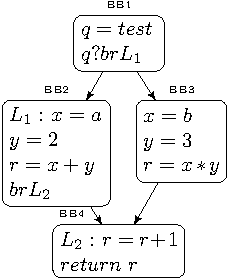
\includegraphics{specul}
    \label{fig:orig}}

  \subfloat[with basic block ordering] {
     \begin{tabular}[t]{lllll}
      & ALU1 & ALU2 & ALU3 & ALU 4 \\
\hline
      & $q = test$         &   -     &   -   & - \\
      & $q \cond br$ $L_1$ & -       & - & - \\
      & $x = 2$            & $y = 3$ & - & - \\
      & $r = x * y$ & - & - & - \\
$L_2$ & $r = r + 1$ & - & - & - \\
      & $return$ $r$ & - & - & - \\
$L_1$ & $x = a$ & $y = 2$ & - & - \\
      & $r = x + y$ & - & - & - \\
      & $br$ $L_2$ & - & - & - \\
     \end{tabular}}
\vspace{1cm}
  \subfloat[After if-conversion] {
     \begin{tabular}[t]{lllll}
      & ALU1 & ALU2 & ALU3 & ALU 4 \\
\hline
      & $q = test$ & - & - & - \\
      & $x_1 = 2$ & $y_1 = 3$ & $x_2 = a$ & $y_2 = 2$ \\
      & $r_1 = x_1 * y_1$ & $r_2 = x_2 + y_2$ & - & - \\
      & $r = q \cond r_1 : r_2$ & - & - & - \\
      & $r = r + 1$ & - & - & - \\
      & $return$ $r$ & - & - & - \\
      & & & & \\     
      & & & & \\     
      & & & & \\     
      & & & & \\     
     \end{tabular}}
\caption{Static schedule of a simple region on a 4 issue processor}
\label{fig:example1}
\end{figure}

After if-conversion the execution path is reduced to 6 cycles with no branches, regardless of the test outcome, and assuming a very optimistic 1 cycle branch penalty. 

From this introductory example, we can observe that the transformation implies:

\begin{itemize}
\item The merge of execution paths into a single execution path, implying a  better exploitation of available resources.  
\item The reduction of the schedule height, because instructions can be speculated before the branch.
\item That the variables need to be renamed, producing new data dependencies.
\item The introduction of a \textit{merge} pseudo operation.
\end{itemize}

% \annotation{Reference join sets; phi-congruence already here?}
Thanks to SSA, the merging point is already materialized in the original control flow as a $\phi$ pseudo operation and register renaming is a basic property of SSA. Given these similarities between SSA and the if-conversion requirements, the transformation to generate if-converted code seems natural. We describe here the framework to exploit those properties on larger scale control flow regions.

\subsection{Architectural requirements}

The \textit{merge} pseudo operations needs to be mapped to a conditional form of execution in the target's architecture. Figure \ref{fig:pred} shows different models of conditional execution.

\begin{itemize}
\item Predicated execution by mean of architectural features that allow an instruction to be executed conditionally by mean of a predicate operand.
\item Speculative execution by mean of conditional moves or $select$ instructions, using temporary registers. 
\item A partial predication model can be used to predicate only a subset of the ISA, usually memory operations that are not easily speculated. Other instructions are speculated.
\end{itemize}

\begin{figure}
\footnotesize
\begin{minipage}[t]{3cm}
\mbox{fully predicated} \\
$p \cond x = a + b $ \\
$\overline{p} \cond x = a * b $ \\
\end{minipage} 
\begin{minipage}[t]{3cm}
\mbox{select} \\
$t_1 = a + b $ \\
$t_2 = a * b $ \\
$x= p \cond t_1 : t_2 $ \\
\end{minipage}
\begin{minipage}[t]{3cm}
\mbox{cmov} \\
$x = a + b $ \\
$t = a * b $ \\
$x = cmov p,t$ \\
\end{minipage}
\caption{Conditional execution using different models}
\label{fig:pred}
\end{figure}

To be speculated, an instruction must not potentially create any side effects, or hazards. For instance a memory load must not trap. This prevents the conditional execution by means of speculation of memory access for which the address is valid only on the selected path. Other reasons are may-alias problems during the memory instructions layout. Memory operations are therefore a major impediment to if-conversion. This is regrettable, because as long latency operations, speculative loads can be very effective to fetching data earlier in the instruction stream, reducing stalls. Modern architectures provide architectural support to dismiss invalid address exceptions. Examples are the $ldw.d$ dismissible load operation of the $ST231$ or $multiflow$ processors or the $IA64$ speculative loads. The main difference is that with a dismissible model, invalid memory access exceptions are not delivered, which can be problematic in embedded or kernel environment that relies on memory exception for correct behavior. A speculative model allows catch the exception thanks to the token bit check instruction. Some architectures, like the $IA64$ offer both speculative and predicated memory operations.

\begin{figure}
\begin{minipage}[t]{4cm}
\mbox{IA64 speculative load} \\
$t = ld.s(addr) $ \\
$chk.s $\\
$p \cond x = t$ \\
\end{minipage}
\begin{minipage}[t]{4cm}
\mbox{Multiflow dismissible load} \\
$t = ldw.d(addr) $ \\
$x = select\:p \cond t : x $ \\
\end{minipage}
\begin{minipage}[t]{4cm}
\mbox{base store hoisting} \\
$x=select\:p \cond addr : dummy $ \\
$stw (x, value) $ \\
\end{minipage}
\begin{minipage}[t]{4cm}
\mbox{index store hoisting} \\
$index=select\:p \cond i : j $ \\
$stw (x[index], value) $ \\
\end{minipage}
\caption{Examples of speculated memory operations}
\label{fig:spec}
\end{figure}

Stores can also be executed conditionally by speculating part of their address value, with additional constraints on the ordering on the memory operations due to possible alias between the two paths. Figure \ref{fig:spec} shows examples of various form of speculative memory operations.

We first start to describe the structural selection of a set of CFG regions. We then describe the operations necessary to assign the instructions with their defining predicate. Finally we propose a global framework to pull together those techniques, incrementally enlarging the scope of the if-converted region to its maximum beneficial size.

Note that the $select$ operation is a real instruction that does not need to be replaced during the out-of-SSA phase. If the target architecture does not provide such an instruction to switch between two speculated instructions, it can be emulated using two conditional moves. One advantage to generate $select$ instruction at this stage is that the program stays in full SSA form and that it make all the data dependencies explicit, and can be feed to all SSA optimizers. 

In the remaining of this chapter, We use the notation $r = c \cond :r_1:r_2$, to represent a $select$ like operation resulting of the merge of the result of the speculative execution of the instructions defining $r_1$ and $r_2$. $r$ takes the value of $r_1$ if $c$ is True, else $r_2$. We use the notation $r = c \cond op$ to represent the predicated execution of $op$ if the predicate $c$ is True. $r = \overline{p} \cond op$ if the predicate $c$ is False.

\section{Basic Transformations}

\subsection{SSA operations on Basic Blocks}

\begin{figure}[h]
\centering
  \subfloat[phi removal] {
  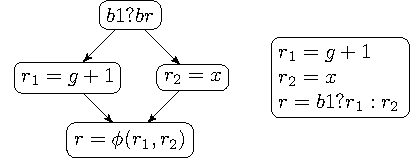
\includegraphics[scale=0.8]{phi_removal}
  \label{fig:phi_rem}}
  \subfloat[phi reduction] {
  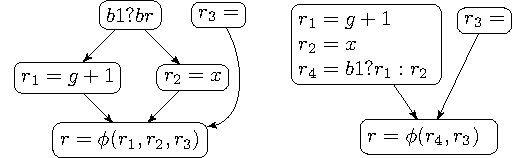
\includegraphics[scale=0.8]{phi_reduction}
  \label{fig:phi_red}}

  \subfloat[phi augmentation $\rightarrow$ (b)] {
  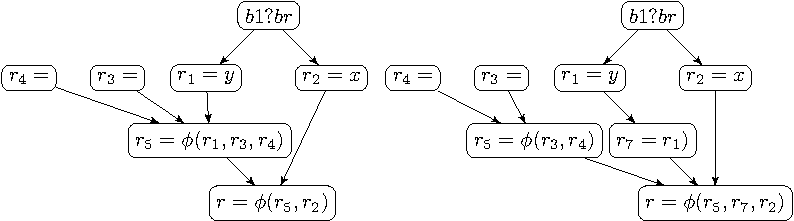
\includegraphics[scale=0.8]{phi_augmentation}
  \label{fig:phi_aug}}

  \subfloat[convergent conjunctive merge $\rightarrow$ (a)] {
  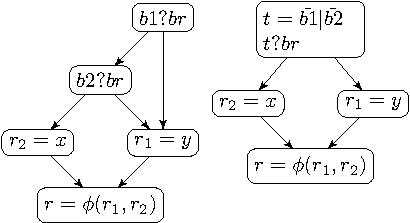
\includegraphics[scale=0.8]{phi_merge}
  \label{fig:phi_merge}}

\caption{local transformations in SSA}
\label{fig:phi_operations}
\end{figure}

The structural if-conversion analysis is based on hammock graphs. A hammock is a single block entry single block exit control flow region $H$ with a distinguished entry node $e$ in $H$ and a distinguished exit node in $H$. We only need to consider the minimal hammock graph of $H$, which is the smallest hammock sub-graph containing $e$. Any other nested depth level of hammocks will be optimized by construction.

Structured programming can produce more sophisticated control flows, we describe later restructuring techniques to isolate the candidate region, and remove problematic edges, such as tail duplication, basic block duplication or conjunctive blocks merging. 

In a first time, we restrict the transformation to the speculative and conditional move model.

Consider a conditional branch depending on a predicate $p$ and a region starting at $BBhead$. Let $BBp$ be the set of single exit basic blocks $(BBi,\dots,BB_n)$ that are on the taken path if $p$ is true and $BBq$ be the set of single exit basic blocks $(BBj,\dots,BB_m)$ that are executed if $p$ is false. The merge point of the if-converted region is at $BBjoin$. We distinguish four types of basic SSA transformations:

\subsubsection{$\phi$ removal} (figure \ref{fig:phi_rem})
The join node of the considered region has two predecessors and the $\phi$ instructions are of the form $r=\phi(r_1,r_2)$. After speculation of $r_1$ and $r_2$ the instruction can be rewritten as $r=p?r_1:r_2$.
Once $BBp$ and $BBq$ have been promoted into $BBhead$, $BBjoin$ has $BBhead$ as its unique predecessor, so it is no longer in its dominance frontier. The $\phi$ instruction can then be discarded.

\subsubsection{$\phi$ reduction} (figure \ref{fig:phi_red})
 The join node of the considered region has $n$ predecessors with $\phi$ instructions of the form $r=\phi(r_1,r_i,r_j,\dots,r_n)$. After merging, the $\phi$ operation is rewritten $t=p?r_i,?r_j$. Since $BBjoin$ is still in the dominance frontier of $BBhead$, a new $\phi\:r=\phi(r_1,t,\dots,r_{n-1})$ is redefined with the new definitions. The merging instruction is inserted after the speculated $r_i$ and $r_j$ definitions into $BBhead$.
The join block $E$ has $n$ predecessors with $n > 2$, and $n$ blocks in its dominance frontier if it contains $\phi$s.

\subsubsection{$\phi$ augmentation} (figure \ref{fig:phi_aug})
The objective is to remove incoming edges from the hammock. Consider a join side node with $n$ predecessors among which $p$ is duplicated into $q$.  The join node of the considered region have $\phi$ instructions of the form $r=\phi(r_1,p,r_i,r_j,\dots,r_{n-1})$. The instruction is rewritten $t=select(p,r_i,r_j)$ and \mbox{$r=\phi(r_1,t,q,\dots,r_n)$}. 
The duplicated blocks are new dominators of $BBjoin$ that define new $defs$. These blocks are now in the dominance frontier of $BBjoin$. SSA is maintained with new $\phi$ upgraded with the new reaching points.

The newly structured hammock can now be transformed by $\phi$-reduction. Data flow dependencies are broken so new opportunities for scalar local optimization are exposed, since $r_1$ can be propagated into the $\phi$, simplifying the region analysis.

\subsubsection{Conjunctive predicate merging} (figure \ref{fig:phi_merge})
The regions containing a Basic Block that is reached from two paths can be optimized by merging predicates. Such conjunctive branches can be used to represent logical $and$ or $or$ conditional operations. They can also be defined as two nested hammocks, such that each of them is connected to the other by their conditional basic block. In such a case a normalization pass might be needed to align the branch conditions into logical expression equivalence. Note that the last basic block does not necessary join into a $\phi$. In this case this is a non-convergent predicate merging, that cannot be if-converted until the iterative process constructs the region to a point where the conditional blocks share the same immediate post dominator. XXX TODO example XXX

\subsection{SSA representation of conditional instructions}

One problem of the described SSA-speculative framework is that it does not fit very well with a predicated model of conditional execution. Since $\phi$ instructions are transformed to turn joint points into conditional moves, we should backtrack to transform conditional moves into predicated instructions. This process of transforming speculation into predication introduces a renaming problem: A single register name can have two different assignments (under different predicates), which breaks the SSA property of single static assignment. The solution is express the predicate dependency without speculation and conditional moves, using the $\psi$-SSA representation that converts join points into an extended SSA representation.

In the $\psi$-SSA representation, the edge dependency from the basic block within which the $\phi$ argument defined in the original CFG is replaced by a new data dependency holding the condition. This dependency needs to be materialized as a $select$ or $\psi$ operation.

\begin{figure}
\begin{minipage}[t]{3.5cm}
\mbox{SSA:} \\
$ if (p) $ \\
$   x_1 = a+b $ \\
$ else $ \\
$   x_2 = 0 $ \\
$ x = \phi (x_1, x_2) $ \\
\end{minipage}
\begin{minipage}[t]{3.5cm}
\mbox{SSA-speculative form:} \\
$x_1 = a + b $ \\
$x_2 = 0 $ \\
$x = p \cond  x_1 : x_2$ \\
\end{minipage}
\begin{minipage}[t]{3.5cm}
\mbox{$\psi$-SSA form:} \\
$x_1 = a + b $ \\
$x_2 = 0 $\\
$x = \psi (p \cond x_1, \overline{p} x_2) $ \\
\end{minipage}
\end{figure}

Note that unlike $\phi$ arguments that are considered simultaneously (they do not depend upon each other), $\psi$ arguments are executed sequentially and ordered from their definition predicate set. This property is necessary because of the new data dependencies introduced into the straight line of the predicated code stream.

The basic alternative behind the SSA transformations is to either replace the instructions defining the $\phi$ pseudo instructions by equivalent predicated instructions merging into $\psi$ pseudo instruction, or speculate the instructions then merging into a $select$ equivalent instruction, removing the $\phi$, while maintaining the SSA properties.

\subsection{Predicate assignment in SSA}

In SSA form, we distinguish two kinds of speculative execution. Unconditional speculation is the speculation of an instruction where the result operand does not appear as a $\phi$ operand. Conditional speculation is the execution of an instruction where the result merge into a $\phi$ operand inside the hammock. The instructions can be predicated or speculated but in addition the result need to be realized into the merging operation.

\begin{figure}[h]
\centering
  \subfloat[minimal if-conversion] {
   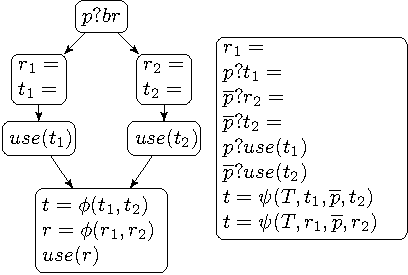
\includegraphics[scale=0.7]{phi_min}
   \label{fig:phi_minimal}}
  \subfloat[pruned if-conversion] {
  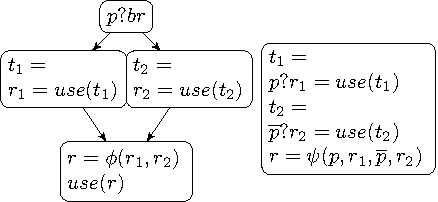
\includegraphics[scale=0.7]{phi_pru}
  \label{fig:phi_pruned}}
\caption{SSA predicate minimality}
\label{fig:minimality}
\end{figure}

The minimality of the SSA region determines the ability to assign a minimal predicate to the instructions. In Minimal SSA-see chapter~\ref{chap:properties_and_flavours}-, $\phi$ functions might be inserted for variables that have a live range limited to the if-converted region, and might be temporaries. As pictured in figure \ref{fig:phi_minimal} the number of $\phi$ instructions will determine the number of instructions that will be assigned a predicate, and thus the minimality of the if-converted region in term of number of predicated instructions. In pruned SSA \ref{fig:phi_pruned}, the variables are not $\phi$ related, so they do not need to be connected through a predicate. In this respect; pruned SSA exposes the smallest number of predicate dependencies, giving more freedom for scheduling and register allocation. Note that those predicates could be optimized later by predicate promotion, but this would locally introduce deficiency in the cost functions.

To identify the operation's results that need to be conditionally defined, we only need to look at the defining instructions of the $\phi$ instructions. All temporaries that do not have a join point within the considered region and that don't have a side effect can be unconditionally speculated during the SSA transformation processes. Only instructions with a side effect need to be guarded. 
Instruction predicates from the taken path are merged (using a logical and) with the branch parameter. Predicates in instructions from the fall trough path are merged with the complement of the branch parameter.

The process is applied iteratively on the CFG in SSA form until no more reductions are possible. The quality of the SSA taken as input does not affect the correctness of the algorithm: if the control flow is in pruned SSA, i.e two paths $x->+z$ and $y->+z$ converge at node z, then a $\phi$ node is inserted at z only if z is alive in or after z. in which case x and y can be promoted and no merging operation is needed. 

\subsubsection{Partial redefinition}

A $\psi$ operation exposes new data dependencies, by expressing the merge of two definitions. Note that the order of the partial definition is important, because a definition partially redefines the preceding ones. We use this property to speculate the first definitions, so it becomes speculated instead of disjoint. This local optimization allows the removal of predicate dependencies but also creates a new partial dependency when predicates are not disjoint. 

\begin{figure}
\footnotesize
\begin{minipage}[t]{4cm}
\mbox{disjoint predicates} \\
$ p = test $ \\
$ p \cond x_1 = a + b $ \\
$ \overline{p} \cond x_2 = c $ \\
$ x = \psi(p \cond x_1, \overline{p} \cond x_2) $ \\
\end{minipage}
\begin{minipage}[t]{4cm}
\mbox{optimized order predicates} \\
$ x_1 = a + b $ \\
$ p = test $ \\
$ \overline{p} \cond x_2 = c $ \\
$ x = \psi(T \cond x_1, \overline{p} \cond x_2) $ \\
\end{minipage}
\end{figure}

$T$ represents the $True$ predicate. This optimization is useful to save one predicate register and to remove a data dependency between a predicate definition and its use. 
The $\psi$ definition is defined on the $T$ predicate set, therefore it is speculable, as shown in next paragraph.

\subsubsection{$\psi$ speculation properties}

Since $\psi$ operations are part of the intermediate representation, they can be considered for inclusion in a candidate region for if-conversion. The conditional operations that they refer can in turn be speculated or predicated iteratively. We define here the promotion rules for $\psi$ operands, whereas the instructions defining the $\psi$ operands will be speculated.

Consider the instructions \ref{nested_psi} containing a sub region already processed. The $\psi$ operation can be safely speculated if all the instructions defining its operands can be speculated: they don't produce hazardous execution, they don't produce any side effects and there exists a conditional move instruction to merge the operands. Then the block can be executed regardless of the value of $c$. The use of the $\psi$ result is also unconditionally executed.

\subsubsection{$\psi$ predication properties}

If an instructions is not speculable, it must be predicated:
In \ref{nested_psi_predicated}, the $c$ condition merges with all conditions under which the $\psi$ operands are defined. Here a new predicate $p_1$ is created to hold the predicate definition for the instructions defined under $c$. 

Note that conceptually, the speculative $\psi$ execution allows a predicate definition domain larger that the original one, such that the predicative transformation exactly matches the initial definition domain, at the expense of more data dependencies and predicate computation.

We can see with this example that the decision to speculate or predicate can be done at the level of each joining definition, allowing a mix of both speculation and predication. The advantage of speculation over predication is a reduced dependency length. The disadvantage of speculation is that it increases register pressure until the merge point, and potentially moves long latency operations on the critical path.
 
\begin{figure}
\footnotesize
\subfloat[nested if] {
\begin{minipage}[b]{3.5cm}
$ if (c) $ \\
$ \{ $ \\
\hspace*{2mm}$ x_1 = a + b $ \\
\hspace*{2mm}$ \overline{p} \cond x_2 = c $ \\
\hspace*{2mm}$ x = \psi(T \cond x_1, \overline{p} \cond x_2) $ \\
\hspace*{2mm}$ d_1 = use (x) $ \\
$ \} $ \\
$ else $ \\
\hspace*{2mm}$ d_2 = 3 $ \\
$ d = \phi(d_1,d_2) $ \\
\end{minipage}
\label{nested_psi}}
\subfloat[speculated nested] {
\begin{minipage}[b]{3.5cm}
$ x_1 = a + b $ \\
$ \overline{p} \cond x_2 = c $ \\
$ x = \psi(T \cond x_1, \overline{p} \cond x_2) $ \\
$ d_1 = use (x) $ \\
$ \overline{c} \cond d_2 = 3 $ \\
$ d = \psi(T \cond d_1, \overline{c} \cond d_2) $ \\
\end{minipage}
\label{nested_psi_speculated}}
\subfloat[predicated nested] {
\begin{minipage}[b]{3.5cm}
$ q = \overline{p} \& {c} $ \\
$ c \cond x_1 = a + b $ \\
$ q \cond x_2 = c $ \\
$ x = \psi(c \cond x_1, q \cond x_2) $ \\
$ c \cond d_1 = use (x) $ \\
$ \overline{c} \cond d_2 = 3 $ \\
$ d = \psi(c \cond d_1, \overline{c} \cond d_2) $ \\
\end{minipage}
\label{nested_psi_predicated}}
\caption{Inner region $\psi$}
\end{figure}

\section{Global Analysis and Transformations}

Critical regions are rarely just composed of simple if-then-else control flow regions and processors have limited resources. The number of registers will determine the acceptable level of data dependencies to minimize register pressure. The number of predicate registers will determine the depth of the if-conversion so that the number of conditions does not exceed the number of available predicates and the number of processing units will determine the number of instructions that can be executed simultaneously. 

For this reason, standard techniques are either limited to a single conditional branch using peephole-style pattern matching or intrinsic functions (conditional code is inlined by the compiler in the internal representation). A more sophisticated approach is to scope larger regions such as hyperblocks. 

\subsection{Hyperblock formation}

A Hyperblock is a region of straight code with a single entry and possibly multiple exits where inner branches have been removed by if-conversion.
Hyperblocks enlarge the scope for scheduling in two ways. First, since basic blocks swell as the scope of the predicated region grows, static scheduling can now be unconstrained. Second, instructions can be freely speculated without the need for compensation code. Conditional code to exit the hyperblock does not impact the execution flow, using a proper code basic block reordering to favor fall through execution.

Tail duplication is used to exclude from the Hyperblock basic blocks that cannot be if-converted, either because they contain hazardous instructions, or because of heuristic decisions. 

Standard approach to Hyperblock construction is to apply the following steps:

\begin{itemize}
\item Create a trace and select the blocks. A trace is a sequence of basic blocks that can be scheduled together. 
\item Remove the side entries with tail duplication. This step removes the scheduling constraints imposed by side entries.
\item Perform if-conversion while still in SSA.
\end{itemize}

\subsection{CLassical approach}

One way to perform if-conversion in SSA is to apply a classical if-conversion algorithm, such as Fang \cite{Fang:1996:CAI:645674.663446} or RK \cite{Schlansker-predicated}, on a conventional SSA representation. 
During the if-conversion process, instructions that are merged into the deleted $\phi$ operations are now expressed as $\psi$ operations, merging different values from their $\psi-congruence$ class. Assuming that all instructions are predicated, an additional pass is required during instruction selection to emit speculative instructions when a predicated variant is not available. Another pass is needed for predicate promotion, based on the predicate dependence graph.

To illustrate the differences between a traditional framework and a native SSA framework, we first start by describing the RK algorithm proposed by Park and Schlansker on the nested tests in figure \ref{fig:nested1}. We will then describe in detail the SSA based approach.

Standard if-conversion techniques address the problem in the following order: first, identify the region to be if-converted. An execution trace is selected based on profiling information to isolate the region. Then allocate boolean variables to the basic blocks, in the identified region. Then perform predicate initialization placement, instruction emissions and CFG restructuring into the final if-converted regions.

The RK algorithm starts by computing the Control Dependence Graph. It is necessary to associate each basic block with a guard condition, and to associate each guard width the set of basic blocks that need to set it. The algorithm creates a new guard, eventually initialized to false, for each condition. \ref{fig:nested2} shows the inner basic blocks with the new conditions initialized, and \ref{fig:RK} the RK mappings.

\begin{figure}
\centering
  \subfloat[Nested test] {
    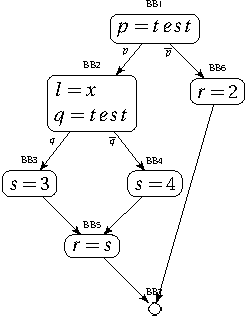
\includegraphics[scale=0.8]{nested1}
    \label{fig:nested1}}
  \subfloat[Predicate Assignments] {
    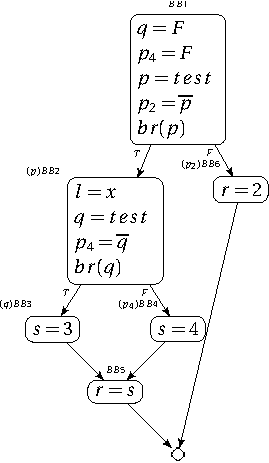
\includegraphics[scale=0.8]{nested1_rk}
    \label{fig:nested2}}
  \subfloat[After Instruction layout] {
    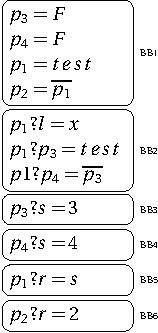
\includegraphics[scale=0.8]{nested1_rk2}
    \label{fig:nested}}
\caption{Classical support for partial predication}
\label{fig:trad_part_pred}
\end{figure}

\begin{figure}
\footnotesize
  \subfloat[R mapping] {
     \begin{tabular}[t]{|l|cccccc|}
\hline
      Basic Block & BB1 & BB2 & BB3 & BB4 & BB5 & BB6  \\
\hline
      Guard       &  T  &  p   & q  & p4  &  p  &  p2 \\
\hline
     \end{tabular}}
  \subfloat[K mapping] {
     \begin{tabular}[t]{|l|cccc|}
\hline
      Guard          & p & q & p4  & p2  \\
\hline
      Basic Block    & 1 & 2,-0 & -2,-0 & -1 \\
\hline
     \end{tabular}}
\caption{Output from RK algorithm}
\label{fig:RK}
\end{figure}

By the end, the algorithm merges the basic blocks, using the predicates and the conditionalized instructions, and removes the instruction branches. \ref{fig:nested}. 

This approach assumes that the region to if-convert is defined and that all instructions can be predicated, Without predicate support for comparison instructions, logical operations must be used to merge condition setting operations. For instance, in the given example, the initialization sequence $p_1 ? p_3=test$ needs to be rewritten as $t=test; p_1=p_3 \& t$. An algorithm based on speculative transformations, necessary to support partially predicated architectures, is then penalized by this approach, since an additional pass is needed to convert a conditional instruction into a temporary register and a conditional move.

We describe next how hyperblocks are now built under SSA, in which the if-conversion process is inherently part of a single comprehensible framework.

\subsection{SSA Iterative if-conversion algorithm}

For each basic block considered within the region, a predicate must be computed and assigned to the corresponding instructions. Those predicate computations introduce new instructions and new data dependencies, that need to be controlled while the region that is been if-converted.

The native If-conversion in SSA form is based on an iterative, incremental if-conversion construction, unifying region selection and region transformation. 

The algorithm takes as input a structured region in SSA form and produces a valid SSA representation using conditional move instructions to realize join points, Incrementally building-up the if-converted region during a control flow traversal using a native SSA framework.

To perform translation from a structured control flow region, we iterate through the basic blocks in post-order traversal to create the list of candidate conditional blocks of the control flow. Post-order traversal guarantees that each inner region will be processed before regions of larger scope. No sub-graph needs to be selected at this point, because the decision to if-convert will be retaken incrementally from inner to outer regions as the hyperblock grows. When the region cannot grow anymore because of resources, or because a basic block cannot be if-converted, then another region is considered in the post-order list. When all the control flow is explored, the process is restarted until no more reduction is possible.

During this incremental process, since nested regions are already predicated when evaluating the if-conversion of a branch, all side effects introduced by the if-conversion, such as new predicate merging instructions, new conditional moves merging flow or new data dependencies, will be accounted for locally. Furthermore, the predicate assignment is simplified, since new predicates are mechanically inserted when merging inner regions containing conditional code. The prevalent idea is that the inner region once predicated will be viewed as a single basic region by the outer scopes evaluation engines.

As the algorithm processes the control flow in post-order traversal, the dominator tree does not change, and it is possible to maintain the SSA locally to the inner region. By recurrence the if-converted region can in turn be optimized out if its head belongs to the dominance frontier of an outer region.

Consider for example the control flow transformations for the $wc$ program (figure \ref{fig:wc1}). The exit node is BB7. Nodes BB7 and BB3 contains XXX TODO finish this XXX

 The post-order list of the basic nested regions is {BB11, BB17, BB16, BB14, BB10, BB9, BB6, BB2}. The head of nested hammocks is represented by circle nodes. The nodes BB3 and BB7 contains calls, so they need to be excluded from the if-conversion algorithm.
The first hammock region starting at BB11 to BB2 contains BB12, promoted such that BB2 becomes the single successor of BB11. 
For the region starting at BB17, BB19 cannot yet be promoted because of the side entry, so it is duplicated into BB15, such that BB15 has now BB2 as successor.
BB16 is the start of a region containing BB17 and BB19. The former can be merged from the 2 conditions coming from BB16 and BB17. BB17 can be promoted into BB16 under BB16's conditions and BB19 under BB16 and BB17 conditions. Note that at this stage BB16's successors are BB19 and BB2.
BB14 is the head of the newly created region where BB15, BB16 and BB17 can be promoted. From BB9 a merging predicate is computed with predicate in BB10. Instructions in BB14 are conditionalized on this new predicate and BB10 promoted, forming a new hammock at BB9 with BB14 and BB11 that can be promoted. The last candidate, BB2 is the start of a region that cannot be promoted, because of the call in BB3.
The region is now if-converted, leaving a single back-edge, removing 7 branches inside the body loop. At this stage, a local decision can be made to decide if tail-call must be performed to form an hyperblock containing only BB2,BB5,BB6 and BB9, excluding BB3. 

\begin{figure}
  \subfloat[Before if-conversion] {
    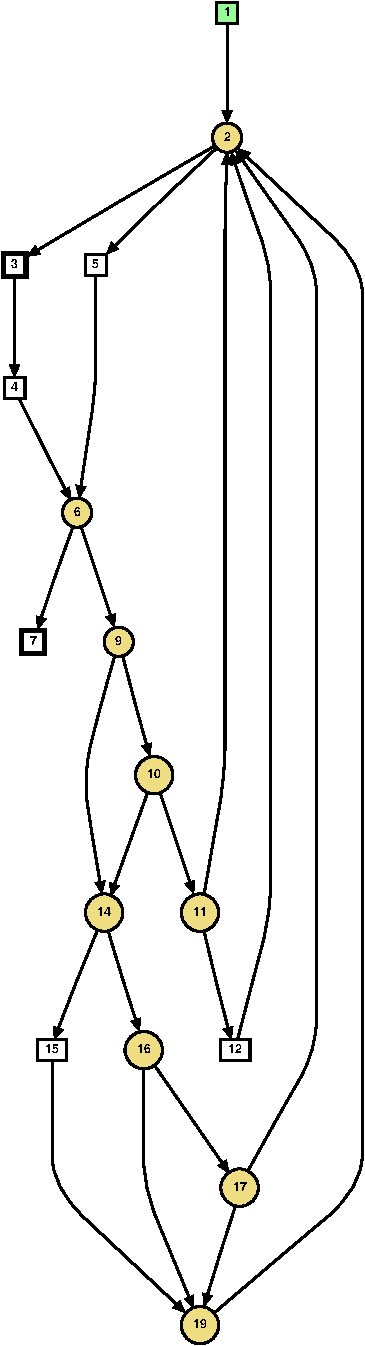
\includegraphics[scale=0.6]{graph1}
    \label{fig:wc1}}
  \subfloat[After if-conversion] {
    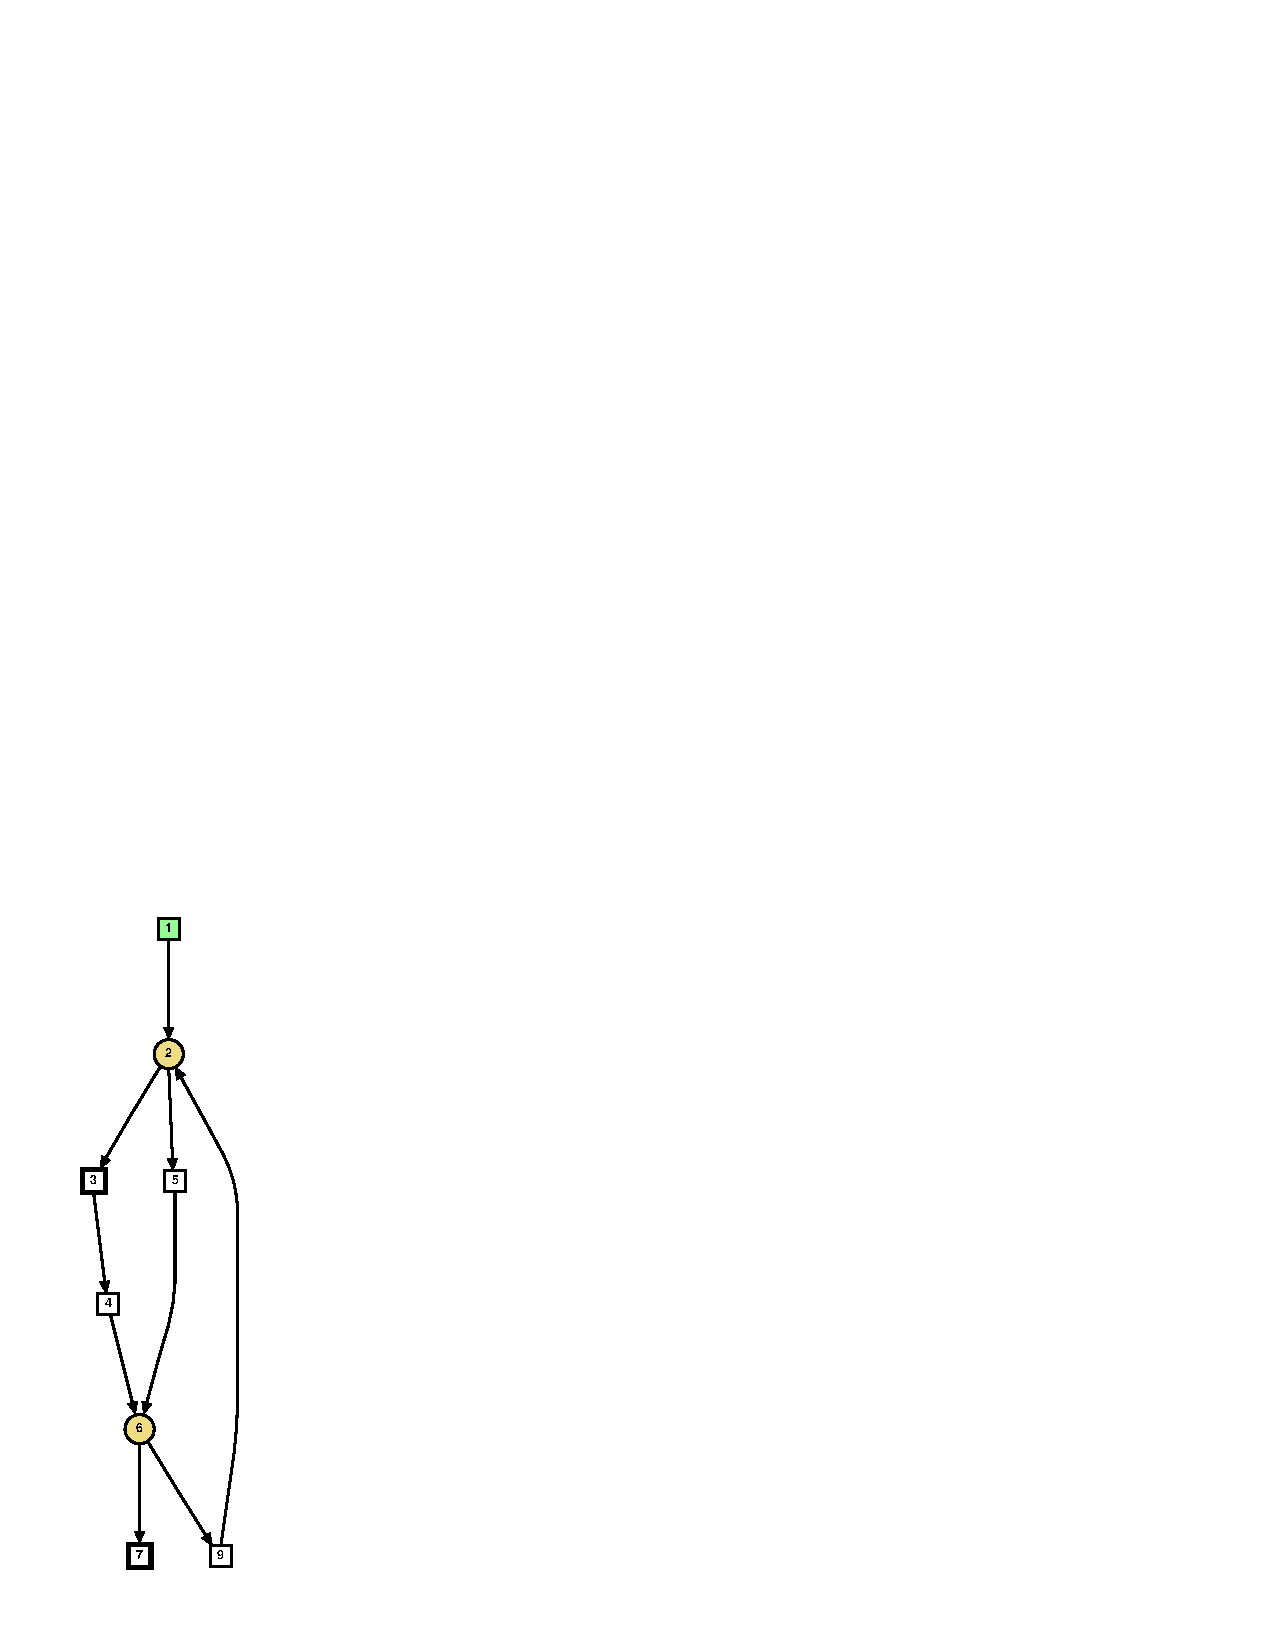
\includegraphics[scale=0.6]{graph7}
    \label{fig:wc2}}
\label{fig:wc example}
\end{figure}

\subsection{Tail Duplication}

Consider the example of Hyperblock formation given in figure \ref{fig:hyper1}. This loop contains two branches, and so if-converting it would be profitable. However, block selection has excluded BB2 and has integrated BB5, because heuristics have determined that the schedule of BB5 inside BB4 would be beneficial. The trace contains {BB1, BB3, BB4, BB5, BB6}. Since BB4 has a side entry, it must be removed by tail duplication. Figure \ref{fig:hyper2} shows the control flow after block duplication. Notice that a new node, BB7, has been added after the tail duplication by a process called branch coalescing. Finally figure \ref{fig:hyper3} shows the code once if-converted.

\begin{figure}[h]
  \subfloat[loop] {
    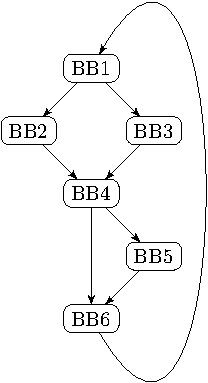
\includegraphics[scale=0.7]{hyper1}
    \label{fig:hyper1}}
  \subfloat[standard tail-duplication] {
    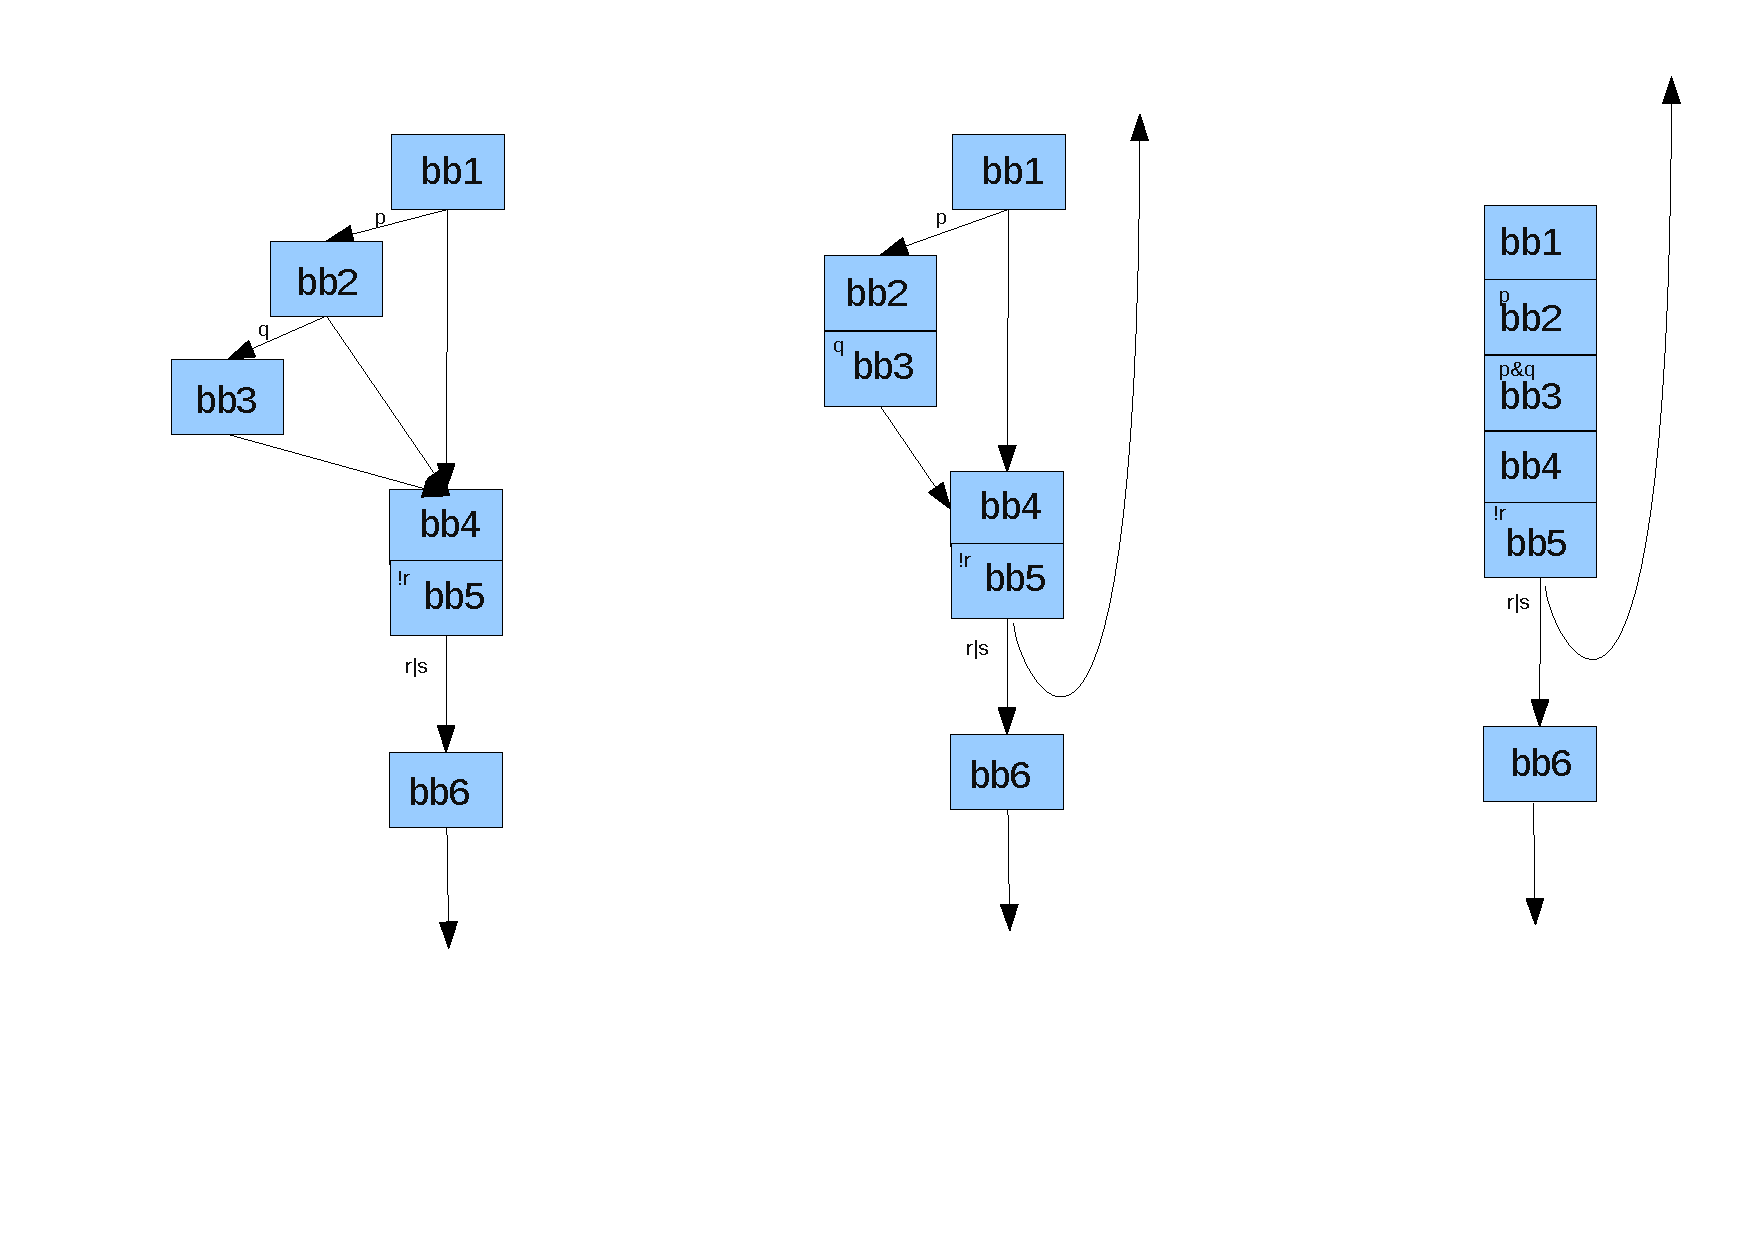
\includegraphics[scale=0.7]{hyper2}
    \label{fig:hyper2}}
  \subfloat[after SSA if-conversion] {
    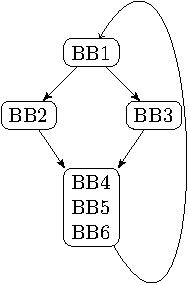
\includegraphics[scale=0.7]{hyper4}
    \label{fig:hyper4}}
  \subfloat[final flow] {
    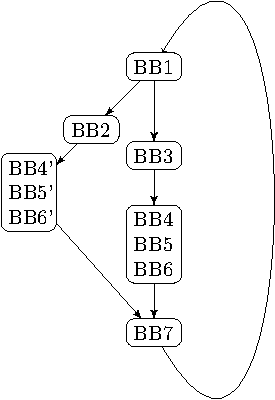
\includegraphics[scale=0.7]{hyper3}
    \label{fig:hyper3}}
\end{figure}

When using this standard decomposition, the if-conversion is performed after tail-duplication. Hyperblock formation, if-conversion and speculation introduce a major phase ordering problem. 

Consider in contrast how tail-duplication can be performed lazily using the SSA iterative transformations, after the code has been if-converted. Figure \ref{fig:hyper4} shows the same loop body where the second $if$ region has been SSA if-converted. The decision to if-convert the region formed by {BB1, BB2, BB3} is now local and can be taken conservatively. Only at this stage, tail-duplication can be performed if necessary to remove the side entry coming from BB2. Duplicating a single predicated block is now a very simple operation that is described in the next paragraph. Note that if BB2 can be included in the region, the whole loop region would have been if-converted.

\subsection{Basic Block duplication}

Basic Block duplication is used to remove side entries and to obviate the constraints on control dependencies. Unless applied carefully, basic block duplication could be the cause of code bloating without performance improvement. However experience has shown that when applied carefully it can be efficient, enabling further scalar optimizations.
Consider figure \ref{fig:bbdup}. Since we are if-converting from the inner most regions, the algorithm first considers the region {BB3,BB4,BB5,BB6 and BB7}, and discards the edge coming from BB2 by duplicating BB6 into BB8. The $\phi$ becomes a move in the duplicated block with a renamed definition. The new $\phi$ operands are updated from the new edge. Note that in the implementation the block does not need to be created during this intermediate step because it will next be promoted into BB3. We have two nested hammocks and the process can be applied iteratively. The dependency that has been removed in the control flow is now expressed as a data dependency between the two $select$ instructions.
Naturally, any number of incoming edges into the duplicated basic block are allowed.

The algorithm to perform SSA basic block duplication is decomposed into:
\begin{itemize}
\item Extract the $\phi$s definitions to be conditionalized from the duplicated block creating a $move$ instruction and a new reduced $\phi$ (or two $move$ instructions if the duplicated block had only two incoming edges).
\item Then the $\phi$s in the tail basic block are augmented with the new definition created by the new repair instruction. If the $\phi$ was live-out after the tail block a move must be inserted to avoid propagating renaming outside of the region considered. 
\item The last step consists of renaming the new definitions to keep the region in SSA form.
\end{itemize}

\begin{figure}[h]
\centering
  \subfloat[Original] {
    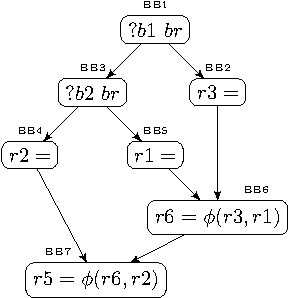
\includegraphics[scale=0.75]{side1}
    \label{fig:side1}}
  \subfloat[After duplication] {
    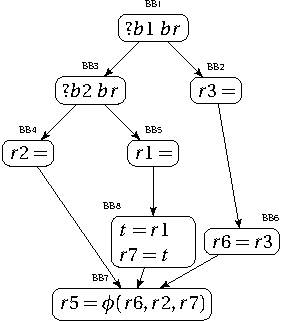
\includegraphics[scale=0.75]{side2}
    \label{fig:side2}}
  \subfloat[inner branch] {
    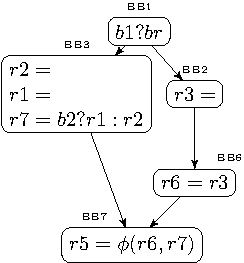
\includegraphics[scale=0.75]{side3}
    \label{fig:side3}}
  \subfloat[outer branch] {
    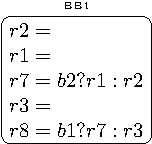
\includegraphics[scale=0.75]{side4}
    \label{fig:side4}}
\caption{Side entry removal using basic block duplication}
\label{fig:bbdup}
\end{figure}

\subsection{Profitability}

Fusing execution paths can over commit the architectural ability to execute in parallel the multiple instructions: Data dependencies and register renaming introduce new register constraints. Moving operations earlier in the instruction stream increases live-ranges. 
Aggressive if-conversion can easily exceed the processor resources, leading to excessive register pressure or moving infrequently used long latencies instructions into the critical path. In a SSA incremental approach, the decision to if-convert or not the inner region will propagate recurrently to the outer regions.

The local decision function to if-convert, or not a inner region in order to enlarge the hyperblock is based on machine model, instructions constraints, execution frequencies. All those form the objective function parameters than will be re-applied locally at each neew transformation.

Since the SSA iterative restructuring framework described earlier reduces the scope for the decision function to a localized part of the control flow graph, the predicate instructions or temporary register to hold the speculated instructions are already in the code that we are considering because the constraints have been resolved. 

Although if-conversion removes branches, it also adds overhead (new instructions to merge predicates, register pressure for speculative conditional, higher dependence height because of the presence of new data dependencies on the predicates).

The prevalent idea is that a region can be if-converted if the cost of the resulting if-converted basic block is smaller than the cost of each region taken separately weighted by the branch frequencies.

We compare the cost of the region before if-conversion. So the cost of a path is the schedule estimation of all the blocks in the path pondered by the execution profile:
\begin{align*}
Cost(path)=Freq(path)*\sum_{k=1}^n(Cost(bb_{k}))
\end{align*}
The cost of the region starting at basic block $head$ before if-conversion is therefore the cost of all the basic blocks in the considered region, on each path.
\begin{align*}
Cost(BBs_{before:\ ifc})=Cost(bb_{head}) + branchlat + Cost(bbs_{taken:\ path}) + Cost(bbs_{fall-though:\ path})
\end{align*}
The Cost after if-conversion is estimated with:
\begin{align*}
Cost(BB_{after:\ ifc})=Cost(bb_{head} \circ bb_{taken:\ path} \circ bb_{fall-though:\ path})
\end{align*}
Where $\circ$ is the composition function that merges basic blocks together, removes associated branches and creates the predicate operations. The resulting $Cost$ applied to the new basic block represents the estimated schedule after if-conversion, that will be effective only if
\begin{align*}
Cost(BBs_{before:\ ifc}) > Cost(BB_{after:\ ifc})
\end{align*}

The cost function needs the target machine description to derive the instruction latencies, resource usage and scheduling constraints. The local dependencies computed between instructions are used to compute the dependence height. The branch frequency is obtained either from static branch prediction heuristics, profile information or user inserted directives.

The estimated cost of the if-converted region is the schedule height estimation of the instructions without the branches. When the schedule height of the if-converted region is smaller than the profiled estimation, then it is profitable.

Register pressure increases due to speculation, because the variables interfere. And the model is restricted to an evaluation of the pseudo register local allocation. Computing the interference graph and simulating a register coalescing process would only take into account local effects, and would lack precision. Consequently this conservative approach might be compensated with aggressiveness factors. The size of the inner region under consideration makes the profitability a sizeable process.

\section{Conclusion} 

We presented in this chapter how an if-conversion algorithm can take advantage of the SSA properties to efficiently assign predicates and lay out the new control flow in an iterative, inner-out process. As opposed to the alternative top-down approach, the region selection can be reevaluated at each nested transformation, using local analysis.
Basic block selection and if-conversion are performed as a single process, hyperblocks being created lazily, using well known techniques such as tail-duplication or branch coalescing only when the benefit is established.
Predication and speculation are often presented as two different alternatives for if-conversion. While it is true than they both require different hardware support, they should coexist in an efficient if-conversion process such that every model of conditional execution is accepted. Thanks to conditional moves and $\psi$ transformations, they are now generated together in the same framework.

\section{Additional reading}

\cite{Rau:2003:IP:1074100.1074489}, exposes ILP in VLIW architectures using trace scheduling and local if-converted if-then-else regions using the $select$ and dismissible load operations. The idea behind was to enable the compiler to statically reorganize the instruction. In this respect, predictability \cite{Fisher:1992:PCB:143371.143493} becomes a major criteria for profitability.

To overcome the hard to predict profitability in conventional if-conversion algorithms, Reverse if-conversion was proposed in \cite{August:1999:PRI:326224.325595}, reconstructing the control flow at schedule time, after application of more aggressive region selection criteria.

Hyperblocks \cite{Mahlke:1992:ECS:144965.144998} was proposed as the primary if-converted scheduling framework, excluding basic blocks which do not justify their inclusion into the if-converted flow of control.

The duality between SSA like $\phi$s and predicate dependencies have been used in other works. In SSA-PS \cite{Jacome01clusteredvliw}, Predicated Switching operations are used to realize the conditional assignments using aggressive speculation techniques with conditional moves. Phi-Predication \cite{Chuang03phi-predicationfor} uses a modified version of the RK algorithm, to map phi-predication with phi-lists, holding guard and topological information. In both works, the use of SSA aims at solving the multiple definition problem exploiting variable renaming and join points, but they are based on speculation using conditional moves. 

In \cite{Stoutchinin_Gao_2004}, $\psi$ instructions are inserted while in SSA using a modified version of the classical Fang algorithm \cite{Fang:1996:CAI:645674.663446}, enabling support for a fully predicated ISA.
Those works established that standard if-conversion techniques can be applied to a SSA form using the $\psi$-SSA representation, or light weight $\phi$-SSA generation, but do not yet exploit the native SSA properties to build up the if-converted region.
A global SSA framework was presented \cite{odes_bruel} to support $select$ moves using aggressive speculation techniques, further extended to $\psi$-SSA \cite{ijes_bruel} allowing a mix of speculative and predicated techniques.

\cite{Mahlke95acomparison} evaluates how predicated operations can be performed using an equivalent sequences of speculative and conditional moves, starting from an if-converted region fully predicated. 










